% Table-of-Contents entry for the Advanced Quantum Technologies submission.
% The manuscript-preparation checklist asks for a 50--60 word ToC text together
% with a graphic of 55 mm x 50 mm (or 110 mm x 20 mm); upload this one-page PDF
% alongside the manuscript.  The graphic is built by code/make_figures.py
% (target ``toc``) from the headline sweep.
\documentclass[11pt]{article}
\usepackage{graphicx}
\graphicspath{{../figures/}{figures/}}
\pagestyle{empty}
\setlength{\parindent}{0pt}
\begin{document}

\section*{Table of Contents text}

Calibrated quantum sensors lose accuracy when hardware noise distorts the
statistics their decoder inverts.  A small variational map, trained only on
calibration data at known phases, restores the noisy outcome distribution
before a frozen decoder reads out the phase.  Across four noise channels it
cuts the mean squared phase error by up to 33 decibels, outperforming
zero-noise extrapolation.

\vfill

\section*{Table of Contents graphic (55 mm $\times$ 50 mm)}

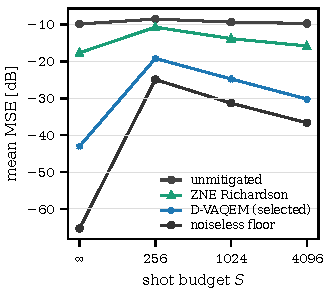
\includegraphics[width=55mm,height=50mm,keepaspectratio]{fig_toc.pdf}

\end{document}
